\documentclass[
  bibliography=totoc,     % Literatur im Inhaltsverzeichnis
  captions=tableheading,  % Tabellenüberschriften
  titlepage=firstiscover, % Titelseite ist Deckblatt
]{scrartcl}

% Paket float verbessern
\usepackage{scrhack}

% Warnung, falls nochmal kompiliert werden muss
\usepackage[aux]{rerunfilecheck}

% unverzichtbare Mathe-Befehle
\usepackage{amsmath}
% viele Mathe-Symbole
\usepackage{amssymb}
% Erweiterungen für amsmath
\usepackage{mathtools}

% Fonteinstellungen
\usepackage{fontspec}
% Latin Modern Fonts werden automatisch geladen
% Alternativ zum Beispiel:
%\setromanfont{Libertinus Serif}
%\setsansfont{Libertinus Sans}
%\setmonofont{Libertinus Mono}

% Wenn man andere Schriftarten gesetzt hat,
% sollte man das Seiten-Layout neu berechnen lassen
\recalctypearea{}

% deutsche Spracheinstellungen
\usepackage[ngerman]{babel}


\usepackage[
  math-style=ISO,    % ┐
  bold-style=ISO,    % │
  sans-style=italic, % │ ISO-Standard folgen
  nabla=upright,     % │
  partial=upright,   % │
  mathrm=sym,        % ┘
  warnings-off={           % ┐
    mathtools-colon,       % │ unnötige Warnungen ausschalten
    mathtools-overbracket, % │
  },                       % ┘
]{unicode-math}

% traditionelle Fonts für Mathematik
\setmathfont{Latin Modern Math}
% Alternativ zum Beispiel:
%\setmathfont{Libertinus Math}

\setmathfont{XITS Math}[range={scr, bfscr}]
\setmathfont{XITS Math}[range={cal, bfcal}, StylisticSet=1]

% Zahlen und Einheiten
\usepackage[
  locale=DE,                   % deutsche Einstellungen
  separate-uncertainty=true,   % immer Unsicherheit mit \pm
  per-mode=symbol-or-fraction, % / in inline math, fraction in display math
]{siunitx}

% chemische Formeln
\usepackage[
  version=4,
  math-greek=default, % ┐ mit unicode-math zusammenarbeiten
  text-greek=default, % ┘
]{mhchem}

% richtige Anführungszeichen
\usepackage[autostyle]{csquotes}

% schöne Brüche im Text
\usepackage{xfrac}

% Standardplatzierung für Floats einstellen
\usepackage{float}
\floatplacement{figure}{htbp}
\floatplacement{table}{htbp}

% Floats innerhalb einer Section halten
\usepackage[
  section, % Floats innerhalb der Section halten
  below,   % unterhalb der Section aber auf der selben Seite ist ok
]{placeins}

% Seite drehen für breite Tabellen: landscape Umgebung
\usepackage{pdflscape}

% Captions schöner machen.
\usepackage[
  labelfont=bf,        % Tabelle x: Abbildung y: ist jetzt fett
  font=small,          % Schrift etwas kleiner als Dokument
  width=0.9\textwidth, % maximale Breite einer Caption schmaler
]{caption}
% subfigure, subtable, subref
\usepackage{subcaption}

% Grafiken können eingebunden werden
\usepackage{graphicx}

% schöne Tabellen
\usepackage{tabularray}
\UseTblrLibrary{booktabs, siunitx}

% Verbesserungen am Schriftbild
\usepackage{microtype}

% Literaturverzeichnis
\usepackage[
  backend=biber,
]{biblatex}
% Quellendatenbank
\addbibresource{lit.bib}
\addbibresource{programme.bib}

% Hyperlinks im Dokument
\usepackage[
  german,
  unicode,        % Unicode in PDF-Attributen erlauben
  pdfusetitle,    % Titel, Autoren und Datum als PDF-Attribute
  pdfcreator={},  % ┐ PDF-Attribute säubern
  pdfproducer={}, % ┘
]{hyperref}
% erweiterte Bookmarks im PDF
\usepackage{bookmark}

% Trennung von Wörtern mit Strichen
\usepackage[shortcuts]{extdash}

\author{%
  Vincent Wirsdörfer\\%
  \href{mailto:vincent.wirsdoerfer@udo.edu}{authorA@udo.edu}%
  \and%
  Joris Daus\\%
  \href{mailto:joris.daus@udo.edu}{authorB@udo.edu}%
}
\publishers{TU Dortmund – Fakultät Physik}


\begin{document}

\section{Versuchsaufbau}
\label{sec:Versuchsaufbau}

Die in diesem Versuch verwendete Lichtquelle ist ein He-Ne-Laser, welcher einen monochromatischen, linear polarisierten Lichtstrahl erzeugt. Dieser Lichtstrahl 
fällt auf die Oberfläche eines Si-Spiegels, wo er teilweise reflektiert und transmittiert wird. Die Bewegungsfreiheit des Lasers um \qty{90}{\degree} stellt 
sicher, dass sowohl die in der Theorie angesprochene senkrechte und parallel Komponente des E-Vektors bevorzugt werden kann. Ziel ist es, die Veränderung der 
Reflexionsintensitäten bei verschiedenen Einfallswinkeln $\alpha_\text{i}$ zu beobachten. Durch einen Drehteller unter dem Spiegel wird gewährleistet, dass 
dieser hinreichend rotiert werden kann. Die Intensität des reflektiert Lichtstrahls wird unter Zuhilfenahme eines Photoelements gemessen, dessen Kurzschlussstrom 
proportional zur Intensität ist. Um grobe systematische Fehler zu vermeiden, ist das Element an einem schwenkbaren Arm montiert, sodass ggf. nachjustiert werden 
kann, um den Reflexionsstrahl erneut auf den Detektor zu richten. Unten skizziert ist das Ensemble der soeben genannten Gerätschaften.

\begin{figure}
    \centering
    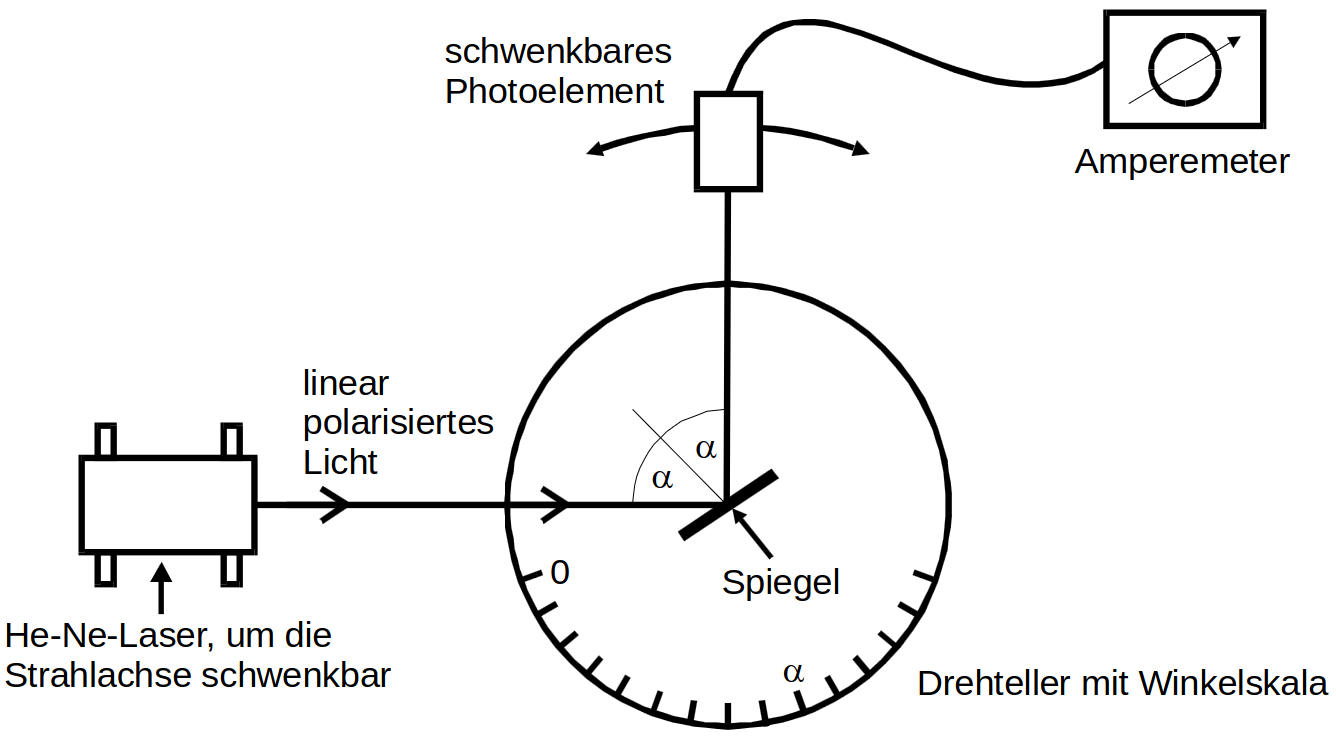
\includegraphics[height=5cm]{Aufbau.png}
    \caption{Skizze des Versuchsaufbaus\cite{Versuchsanleitung_v407}.}
    \label{fig:Versuchsaufbau}
\end{figure}

\section{Versuchsdurchführung}
\label{sec:Durchfuehrung}

Bevor die Reflexionsintensitäten in Abhängigkeit der Winkel gemessen werden können, muss die Messapparatur justiert werden. Hierzu wird zunächst der Probenhalter aus dem 
Strahlengang entfernt, damit der Laserstral direkt zum Detektor gelangen kann. Nach Anbringung des Polarisationsfilters wird der Laser solange gedreht, bis das 
Intensitätsminimum erreicht ist und der Laser befestigt werden kann. Unter maximaler Rotationsamplitude des Schwenkarms wird nun geprüft, ob der Laserstrahl die 
Markierungsstriche des Detektorarms trifft. Ist dies der Fall, kann die Zentriernaden in die Bohrung des Goniometers eingesetzt werden, sodass der Laserstrahl die 
Nadel trifft. Ferner wird kontrolliert, ob die Spiegelfläche tatsächlich senkrecht zur Spiegeloberfläche steht, indem der Laserstrahl unter einem Einfallswinkel von 
\qty{0}{\degree} geworfen wird. Trifft der reflektierte Laserstrahl direkt auf den Laserkopf, so ist eine korrekte Höheneinstellung vorhanden. Abschließend wird die 
Klemmschraube leicht gelöst und der Probenhalter solange gedreht, bis der einfallende Strahl in sich selbst reflektiert. Nachdem die Klemmschraube fixiert ist, kann die 
Messung beginnen.

\begin{figure}
    \centering 
    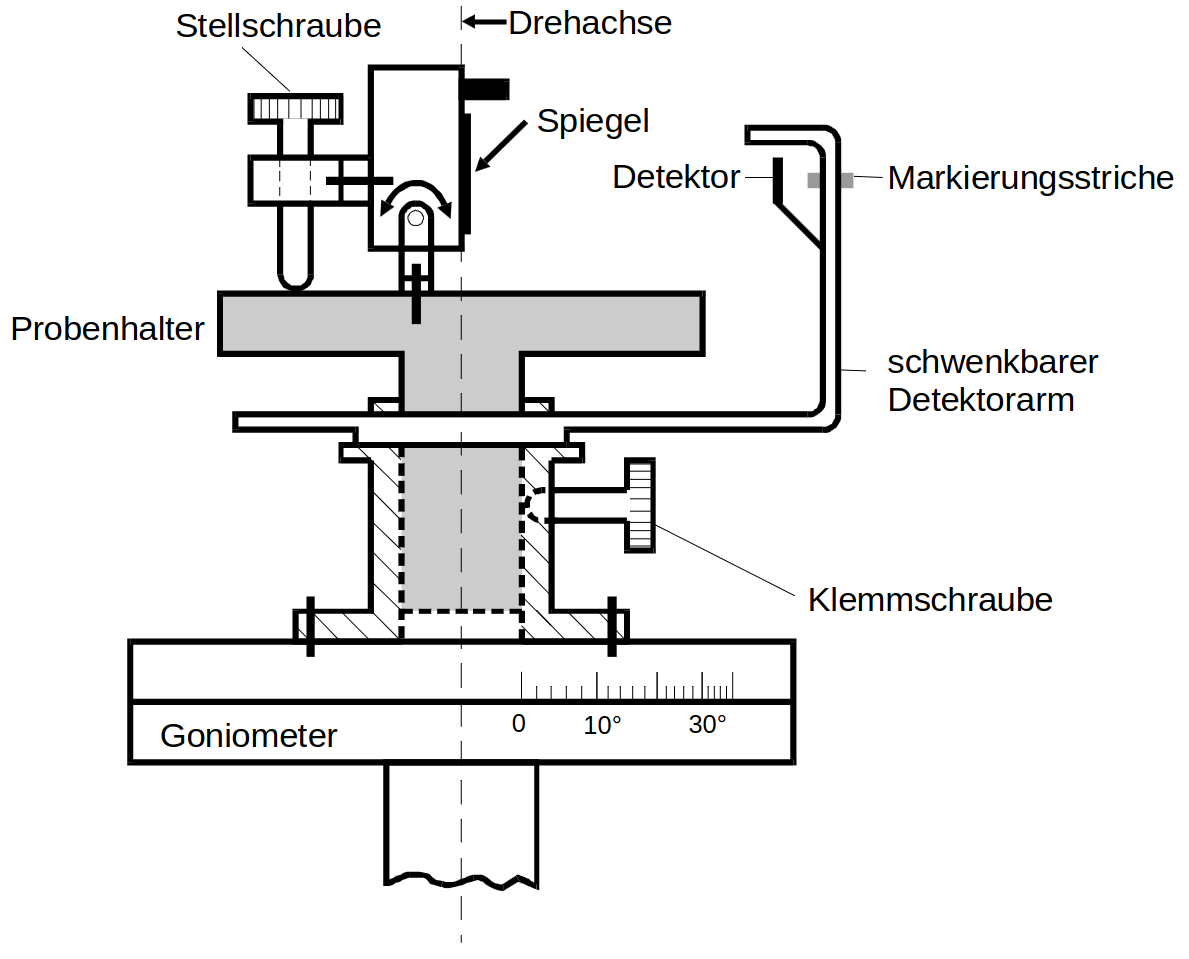
\includegraphics[height=5cm]{Goniometer.png}
    \caption{Abbildung des Goniometers mit zusätzlichem Probenhalter\cite{Versuchsanleitung_v407}.}
    \label{fig:Goniometer}
\end{figure}

\noindent Wie bereits thematisiert, wird die Winkelabhängigkeit der Reflexionsintensität untersucht. Es wird also mit einem Winkel von \qty{5}{\degree} gestartet und
und der zur Intensität proportionale Kurzschlussstrom des Photoelements notiert. Für den identischen Winkel wird zunächt die Polarisationsrichtung verändert, bevor das 
Goniometer auf den nächsten Winkel eingestellt werden kann. Mit einer Schrittweite von \qty{2}{\degree} wird bis \qty{70}{\degree} verfahren. Zwischen \qty{70}{\degree}
und \qty{80}{\degree} wird jeder ganzzahlige Winkel untersucht, um einen präziseren Rückschluss auf den Brewsterschen Winkel treffen zu können. Ist das Rotationsmaximum 
erreicht, so sind alle möglichen Werte für die senkrechte und parallele Polarisation ins Experimentierheft übertragen. Schließlich wird die einfallende Lichtintensität 
$I_\text{e}$ gemessen, indem der Probenhalter entfernt wird und die direkte Lichtintensität auf den Detektor bestimmt wird. Um weiteren systematischen Fehlern vorzubeugen
wird der Dunkelstrom, also der Nettostrom, welcher durch Lichtumwelteinflüsse entsteht, bei ausgeschaltetem Laser gemessen.


\section{Messwerte}

Die Messwerte der Reflexionsintensitäten bzw. Kurzschlussströme bei variierendem Winkel lauten wie folgt:

\begin{table}[H]
    \centering
    \sisetup{table-format=1.2}
    \begin{tblr}{
        colspec = {S[table-format=1.0] S S},
        row{1 } = {guard, mode=math},
        }
        \toprule 
        \text{Winkel} \mathbin{/} \unit{\degree} & I_\perp \mathbin{/} \unit{\ampere} & I_\parallel \mathbin{/} \unit{\ampere} \\
        \midrule 
        5   &   (0.69\pm1)\cdot{}10^{-4} & (0.46\pm1)\cdot{}10^{-4} \\ 
        7   &   (0.40\pm1)\cdot{}10^{-4} & (0.40\pm1)\cdot{}10^{-4} \\ 
        9   &   (0.64\pm1)\cdot{}10^{-4} & (0.44\pm1)\cdot{}10^{-4} \\ 
        11  &   (0.64\pm1)\cdot{}10^{-4} & (0.44\pm1)\cdot{}10^{-4} \\   
        13  &   (0.55\pm1)\cdot{}10^{-4} & (0.40\pm1)\cdot{}10^{-4} \\  
        15  &   (0.68\pm1)\cdot{}10^{-4} & (0.45\pm1)\cdot{}10^{-4} \\  
        17  &   (0.76\pm1)\cdot{}10^{-4} & (0.45\pm1)\cdot{}10^{-4} \\  
        19  &   (0.78\pm1)\cdot{}10^{-4} & (0.45\pm1)\cdot{}10^{-4} \\  
        21  &   (0.78\pm1)\cdot{}10^{-4} & (0.40\pm1)\cdot{}10^{-4} \\  
        23  &   (0.79\pm1)\cdot{}10^{-4} & (0.44\pm1)\cdot{}10^{-4} \\  
        25  &   (0.74\pm1)\cdot{}10^{-4} & (0.42\pm1)\cdot{}10^{-4} \\  
        27  &   (0.80\pm1)\cdot{}10^{-4} & (0.43\pm1)\cdot{}10^{-4} \\  
        29  &   (0.79\pm1)\cdot{}10^{-4} & (0.42\pm1)\cdot{}10^{-4} \\  
        31  &   (0.79\pm1)\cdot{}10^{-4} & (0.41\pm1)\cdot{}10^{-4} \\  
        33  &   (0.84\pm1)\cdot{}10^{-4} & (0.40\pm1)\cdot{}10^{-4} \\  
        35  &   (0.88\pm1)\cdot{}10^{-4} & (0.38\pm1)\cdot{}10^{-4} \\  
        37  &   (0.25\pm1)\cdot{}10^{-3} & (0.38\pm1)\cdot{}10^{-4} \\  
        39  &   (0.24\pm1)\cdot{}10^{-3} & (0.96\pm1)\cdot{}10^{-4} \\  
        41  &   (0.25\pm1)\cdot{}10^{-3} & (0.34\pm1)\cdot{}10^{-4} \\  
        43  &   (0.27\pm1)\cdot{}10^{-3} & (0.33\pm1)\cdot{}10^{-4} \\  
        45  &   (0.25\pm1)\cdot{}10^{-3} & (0.31\pm1)\cdot{}10^{-4} \\  
        47  &   (0.29\pm1)\cdot{}10^{-3} & (0.29\pm1)\cdot{}10^{-4} \\  
        49  &   (0.29\pm1)\cdot{}10^{-3} & (0.27\pm1)\cdot{}10^{-4} \\  
        51  &   (0.25\pm1)\cdot{}10^{-3} & (0.72\pm1)\cdot{}10^{-4} \\  
        53  &   (0.32\pm1)\cdot{}10^{-3} & (0.70\pm1)\cdot{}10^{-4} \\  
        55  &   (0.31\pm1)\cdot{}10^{-3} & (0.58\pm1)\cdot{}10^{-4} \\  
        57  &   (0.32\pm1)\cdot{}10^{-3} & (0.54\pm1)\cdot{}10^{-4} \\  
        59  &   (0.34\pm1)\cdot{}10^{-3} & (0.40\pm1)\cdot{}10^{-4} \\  
        61  &   (0.35\pm1)\cdot{}10^{-3} & (0.40\pm1)\cdot{}10^{-4} \\  
        63  &   (0.34\pm1)\cdot{}10^{-3} & (0.29\pm1)\cdot{}10^{-4} \\  
        65  &   (0.37\pm1)\cdot{}10^{-3} & (0.25\pm1)\cdot{}10^{-4} \\  
        67  &   (0.38\pm1)\cdot{}10^{-3} & (0.64\pm1)\cdot{}10^{-5} \\  
        69  &   (0.42\pm1)\cdot{}10^{-3} & (0.50\pm1)\cdot{}10^{-5} \\  
        70  &   (0.41\pm1)\cdot{}10^{-3} & (0.38\pm1)\cdot{}10^{-5} \\  
        71  &   (0.44\pm1)\cdot{}10^{-3} & (0.31\pm1)\cdot{}10^{-5} \\  
        72  &   (0.42\pm1)\cdot{}10^{-3} & (0.62\pm1)\cdot{}10^{-5} \\  
        73  &   (0.44\pm1)\cdot{}10^{-3} & (0.48\pm1)\cdot{}10^{-5} \\  
        74  &   (0.45\pm1)\cdot{}10^{-3} & (0.38\pm1)\cdot{}10^{-5} \\  
        75  &   (0.48\pm1)\cdot{}10^{-3} & (0.42\pm1)\cdot{}10^{-5} \\  
        76  &   (0.49\pm1)\cdot{}10^{-3} & (0.46\pm1)\cdot{}10^{-5} \\  
        77  &   (0.49\pm1)\cdot{}10^{-3} & (0.62\pm1)\cdot{}10^{-5} \\  
        78  &   (0.52\pm1)\cdot{}10^{-3} & (0.32\pm1)\cdot{}10^{-5} \\   
        79  &   (0.52\pm1)\cdot{}10^{-3} & (0.52\pm1)\cdot{}10^{-5} \\  
        80  &   (0.53\pm1)\cdot{}10^{-3} & (0.85\pm1)\cdot{}10^{-5} \\   
        82  &   (0.50\pm1)\cdot{}10^{-3} & (0.44\pm1)\cdot{}10^{-4} \\  
        84  &   (0.50\pm1)\cdot{}10^{-3} & (0.83\pm1)\cdot{}10^{-4} \\   
        86  &   (0.65\pm1)\cdot{}10^{-4} & (0.63\pm1)\cdot{}10^{-4} \\    
        87  &   (0.44\pm1)\cdot{}10^{-5} & (0.52\pm1)\cdot{}10^{-6} \\
        \bottomrule 
    \end{tblr}
    \label{tab:Meswerte}
\end{table}   

\end{document}

